\subsection{Singular Epsilon}
Figure \ref{fig:singular-epsilon} details the breaking points of the LSODA and CVODE solvers as \(p \to 1\) and \(\varepsilon \to 0\). The solvers operate under very strict tolerances \(\texttt{rtol} = \texttt{atol} = 10^{-13}\) with \(N_x=1000\).

As the nonlinearity index \(p\) approaches 1, the diffusion operator becomes highly singular in regions where the spatial gradient is near zero. The regularization parameter \(\varepsilon\) masks this singularity; however, driving \(\varepsilon \to 0\) exposes the numerical integrators to extreme stiffness and severely ill-conditioned Jacobians. The heatmap illustrates that neither solver is universally resilient.

LSODA demonstrates a predictable failure boundary. At highly singular indices (\(p \leq 1.05\)), it consistently encounters catastrophic failures (indicated in red) once \(\varepsilon\) drops below \(10^{-8}\), exiting with the error \lstinline|scipy/integrate/_ivp/lsoda.py:161: UserWarning: lsoda: Repeated convergence failures (perhaps bad Jacobian or tolerances)|.

Yet, at a slightly elevated index of \(p = 1.25\), LSODA manages to integrate the system across the entire regularization sweep down to \(\varepsilon = 10^{-30}\). Nonetheless, this survival comes at a steep computational cost, visibly indicated by the transition into green and yellow execution times as the stiffness intensifies.

CVODE, on the other hand, exhibits a rather erratic failure topology. It generally collapses at \(\varepsilon \le 10^{-12}\) for indices like \(p = 1.25\) and \(p = 1.01\) with the error \lstinline|sundials/src/cvode/cvode.c:1487 [CVode] At t = 4.38156039034776e-09, mxstep steps taken before reaching tout|. However, an anomalous stability pocket exists at \(p = 1.05\). In this regime, CVODE successfully evaluates the physics down to \(\varepsilon=10^{-14}\) without significant time penalties before finally encountering a catastrophic failure at the \(10^{-30}\) extreme.

It is crucial to emphasize that the \texttt{mxstep} failures observed in these collapsing regimes do not represent premature terminations due to restrictive configurations. For all CVODE benchmarks, the maximum internal step limit was deliberately raised to 1,000,000. Exhausting one million steps at microscopic simulation times (e.g., \(t \approx 10^{-9}\)) in mere seconds indicates the solver is not simply progressing slowly. Rather, it is experiencing a genuine nonlinear convergence failure. This mechanism is highly sensitive to the distance of the first evaluation target (\texttt{tout}). Because the domain interior is initialized to zero, the vanishing initial gradient coupled with a small \(\varepsilon\) creates a massive initial diffusion transient. When assigned a distant output target (e.g., \(T = 0.05\)), internal heuristics estimate a proportionally large initial time step \(h_0\). The catastrophically ill-conditioned Jacobian forces the Newton iterations to diverge, trapping the solver in a recursive rejection loop. The step size \(h\) shrinks toward the limits of double-precision arithmetic without meaningfully advancing the clock until the limit is exhausted. Providing a proximate initial \texttt{tout} with evenly spaced checkpoints generally prevents this heuristic overestimation and allows the solver to finish successfully.

\begin{figure}[H]
  \centering
  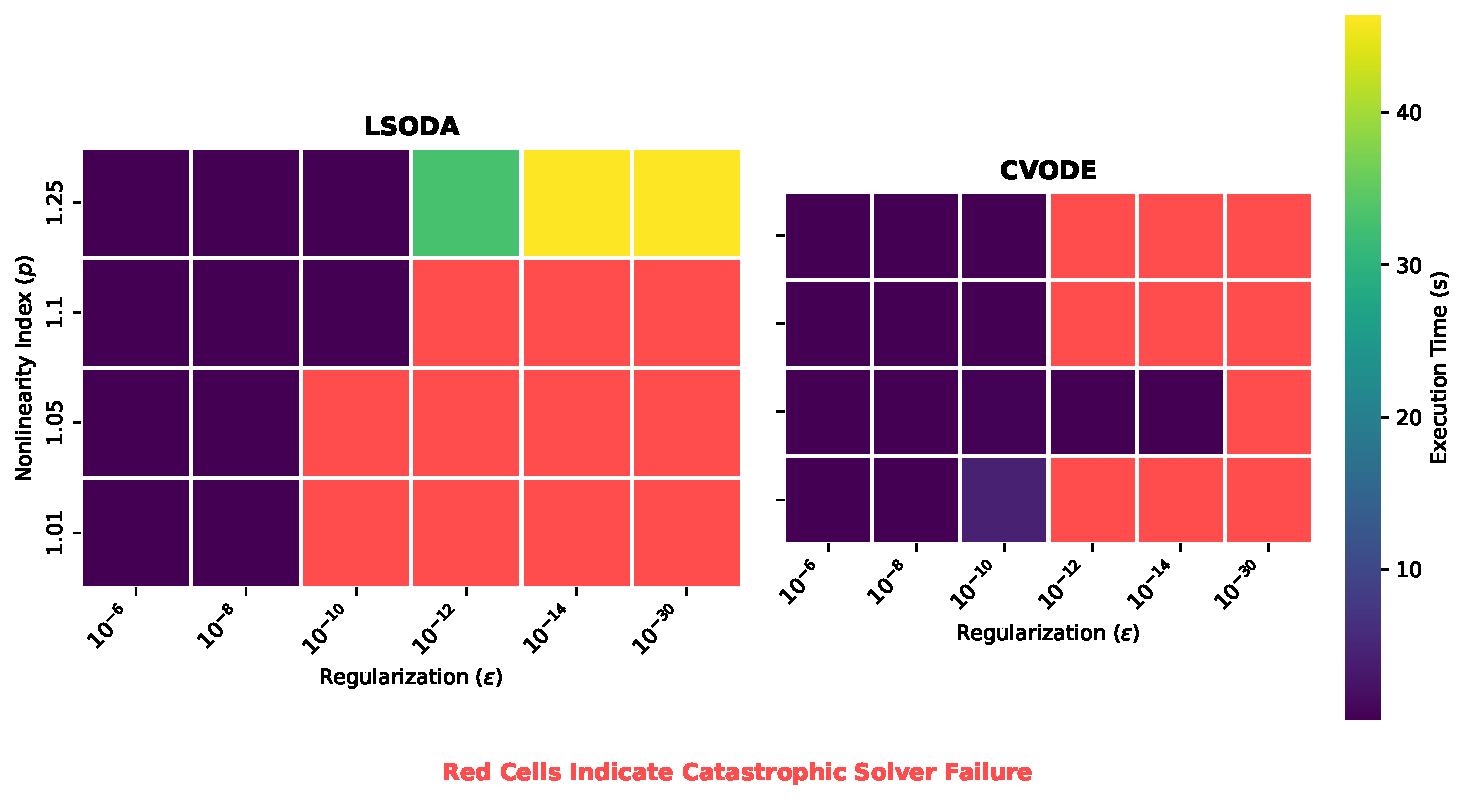
\includegraphics[width=\textwidth]{images/stability_matrix_lsoda_cvode.pdf}
  \caption{Heatmap illustrating execution times and failure boundaries for LSODA and CVODE.}
  \label{fig:singular-epsilon}
\end{figure}

Figure \ref{fig:singular-epsilon-radau} presents the execution time matrix for the Radau solver under substantially harsher conditions. When evaluated at a reduced spatial resolution of \(N_x = 100\) for reasonable computation times, Radau proves extremely robust and stable. Unlike CVODE and LSODA, which would crash even at this reduced spatial resolution, it successfully completes the parameter sweep without convergence failures. However, its remarkably rapid execution times (e.g., \(< 0.5\) seconds for \(\varepsilon \le 10^{-30}\)) are likely a byproduct of its strict L-stability. Upon encountering the stiff initial diffusion, the solver appears to instantly damp the infinite transient, and thus it bypasses the physical resolution of the intermediate dynamics.

\begin{figure}[H]
  \centering
  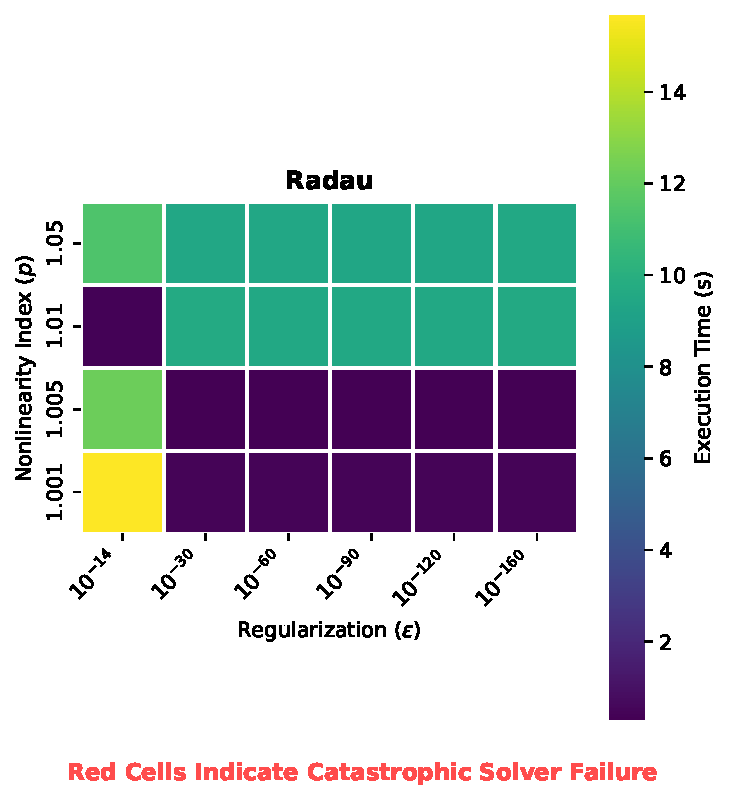
\includegraphics[width=\textwidth]{images/stability_matrix_radau.pdf}
  \caption{Heatmap illustrating execution times for the Radau solver at \(N_x=100\). Darker regions indicate regimes where strict L-stability likely bypassed the initial transient, artificially accelerating execution without integration failure.}
  \label{fig:singular-epsilon-radau}
\end{figure}
